% -*- Mode:TeX -*-

%% IMPORTANT: The official thesis specifications are available at:
%%            http://libraries.mit.edu/archives/thesis-specs/
%%
%%            Please verify your thesis' formatting and copyright
%%            assignment before submission. If you notice any
%%            discrepancies between these templates and the 
%%            MIT Libraries' specs, please let us know
%%            by e-mailing thesis@mit.edu

%% The documentclass options along with the pagestyle can be used to generate
%% a technical report, a draft copy, or a regular thesis. You may need to
%% re-specify the pagestyle after you \include cover.tex. For more
%% information, see the first few lines of mitthesis.cls. 

%\documentclass[12pt,vi,twoside]{mitthesis}
%%
%%  If you want your thesis copyright to you instead of MIT, use the
%%  ``vi'' option, as above.
%%
%\documentclass[12pt,twoside,leftblank]{mitthesis}
%%
%% If you want blank pages before new chapters to be labelled ``This
%% Page Intentionally Left Blank'', use the ``leftblank'' option, as
%% above. 

\documentclass[12pt,twoside]{mitthesis}
\usepackage{lgrind}
%% These have been added at the request of the MIT Libraries, because
%% some PDF conversions mess up the ligatures.  -LB, 1/22/2014
\usepackage{cmap}
\usepackage{color}

\usepackage[T1]{fontenc}

\pagestyle{plain}
\usepackage{url, doi}
\usepackage{hyperref}
% Uncomment to find unused references
%\usepackage{refcheck}

\usepackage{amsmath,amssymb,amsfonts}
\usepackage{algorithm, algorithmic}
\usepackage{booktabs}

%% This bit allows you to either specify only the files which you wish to
%% process, or `all' to process all files which you \include.
%% Krishna Sethuraman (1990).

%\typein [\files]{Enter file names to process, (chap1,chap2 ...), or `all' to process all files:}
\def\all{all}
\ifx\files\all \typeout{Including all files.} \else %\typeout{Including only \files.} \includeonly{\files} \fi

\usepackage{subcaption}
\usepackage{tikz}
\graphicspath{{./anc/}}
\usetikzlibrary{bayesnet, plotmarks, calc}
\usepackage{pgfplots}
\usepgfplotslibrary{groupplots, statistics}
\pgfplotsset{
	compat=1.15,
	table/search path={./anc/},
	only if/.style args={entry of #1 is #2}{
		/pgfplots/boxplot/data filter/.code={
			\edef\tempa{\thisrow{#1}}
			\edef\tempb{#2}
			\ifx\tempa\tempb
			\else
			\def\pgfmathresult{}
			\fi
		}
	}
}

\definecolor{deepblue}{rgb}{0,0,0.75}
\definecolor{deepred}{rgb}{0.6,0,0}
\definecolor{deepgreen}{rgb}{0,0.5,0}

\usepackage{listings}
\lstdefinestyle{mystyle}{%
	basicstyle=\ttfamily\small,
	language=Python,
	morekeywords={self},
	keywordstyle=\color{deepblue},
	emph={BaseMonitor,BaseDriver},
	emphstyle=\color{deepred},
	stringstyle=\color{deepgreen},
	columns=flexible,
	breakatwhitespace=false,
	breaklines=true,
	captionpos=b,
	frame=tb,
	keepspaces=true,
	showspaces=false,
	showstringspaces=false,
	showtabs=false,
	tabsize=1}
\lstset{style=mystyle}

% Tables
\newcommand{\rowgroup}[1]{\hspace{-1em}#1}
% Variables
\newcommand{\vsym}{r}
\newcommand{\tsym}{t}
\newcommand{\msym}{m}
\newcommand{\graph}{G}
% Operators
\DeclareMathOperator{\argmax}{\arg\max}
\DeclareMathOperator{\nhood}{ne}
\DeclareMathOperator{\mrr}{mrr}
\newcommand{\init}{\msym_0}
\newcommand{\curr}{c}
\newcommand{\ival}{\vsym_0}
\newcommand{\itime}{\tsym_0}
\newcommand{\msg}[2]{\msym_{#1 \rightarrow #2}}
\newcommand{\mval}[2]{\vsym_{#1 \rightarrow #2}}
\newcommand{\mtime}[2]{\tsym_{#1 \rightarrow #2}}
\newcommand{\reach}{\msym}
\newcommand{\estreach}{\hat{\msym}}
\newcommand{\card}[1]{\left\vert #1 \right\vert}
% Sets
\newcommand{\contacts}{\mathcal{C}}
\newcommand{\rscores}{\mathcal{R}}
\newcommand{\scores}{\mathcal{S}}
\newcommand{\edges}{\mathcal{E}}
\newcommand{\variables}{\mathcal{V}}
\newcommand{\factors}{\mathcal{F}}
\newcommand{\actors}{\mathcal{G}}
\newcommand{\simpath}{\mathcal{P}}

\begin{document}
% Uncomment to find unnused references
% \nocite{*}
\pagenumbering{roman}
% -*-latex-*-
% 
% For questions, comments, concerns or complaints:
% thesis@mit.edu
% 
%
% $Log: cover.tex,v $
% Revision 1.9  2019/08/06 14:18:15  cmalin
% Replaced sample content with non-specific text.
%
% Revision 1.8  2008/05/13 15:02:15  jdreed
% Degree month is June, not May.  Added note about prevdegrees.
% Arthur Smith's title updated
%
% Revision 1.7  2001/02/08 18:53:16  boojum
% changed some \newpages to \cleardoublepages
%
% Revision 1.6  1999/10/21 14:49:31  boojum
% changed comment referring to documentstyle
%
% Revision 1.5  1999/10/21 14:39:04  boojum
% *** empty log message ***
%
% Revision 1.4  1997/04/18  17:54:10  othomas
% added page numbers on abstract and cover, and made 1 abstract
% page the default rather than 2.  (anne hunter tells me this
% is the new institute standard.)
%
% Revision 1.4  1997/04/18  17:54:10  othomas
% added page numbers on abstract and cover, and made 1 abstract
% page the default rather than 2.  (anne hunter tells me this
% is the new institute standard.)
%
% Revision 1.3  93/05/17  17:06:29  starflt
% Added acknowledgements section (suggested by tompalka)
% 
% Revision 1.2  92/04/22  13:13:13  epeisach
% Fixes for 1991 course 6 requirements
% Phrase "and to grant others the right to do so" has been added to 
% permission clause
% Second copy of abstract is not counted as separate pages so numbering works
% out
% 
% Revision 1.1  92/04/22  13:08:20  epeisach

% NOTE:
% These templates make an effort to conform to the MIT Thesis specifications,
% however the specifications can change. We recommend that you verify the
% layout of your title page with your thesis advisor and/or the MIT 
% Libraries before printing your final copy.
\title{ShareTrace: Contact Tracing with the Actor Model}

\author{Ryan Tatton}
% If you wish to list your previous degrees on the cover page, use the 
% previous degrees command:
%       \prevdegrees{A.A., Harvard University (1985)}
% You can use the \\ command to list multiple previous degrees
%       \prevdegrees{B.S., University of California (1978) \\
%                    S.M., Massachusetts Institute of Technology (1981)}
\department{Department of Computer and Data Sciences}

% If the thesis is for two degrees simultaneously, list them both
% separated by \and like this:
% \degree{Doctor of Philosophy \and Master of Science}
\degree{Master of Science in Computer and Data Sciences}

% As of the 2007-08 academic year, valid degree months are September, 
% February, or June.  The default is June.
\degreemonth{August}
\degreeyear{2022}
\thesisdate{July 31, 2022}

%% By default, the thesis will be copyrighted to MIT.  If you need to copyright
%% the thesis to yourself, just specify the `vi' documentclass option.  If for
%% some reason you want to exactly specify the copyright notice text, you can
%% use the \copyrightnoticetext command.  
% \copyrightnoticetext{\copyright IBM, 1990.  Do not open till Xmas.}

\copyrightnoticetext{}

% If there is more than one supervisor, use the \supervisor command
% once for each.
\supervisor{Erman Ayday}{Assistant Professor}

% This is the department committee chairman, not the thesis committee
% chairman.  You should replace this with your Department's Committee
% Chairman.
\chairman{Vipin Chaudhary}{Chairman, Department Committee on Graduate Theses}

% Make the titlepage based on the above information.  If you need
% something special and can't use the standard form, you can specify
% the exact text of the titlepage yourself.  Put it in a titlepage
% environment and leave blank lines where you want vertical space.
% The spaces will be adjusted to fill the entire page.  The dotted
% lines for the signatures are made with the \signature command.
\maketitle

% The abstractpage environment sets up everything on the page except
% the text itself.  The title and other header material are put at the
% top of the page, and the supervisors are listed at the bottom.  A
% new page is begun both before and after.  Of course, an abstract may
% be more than one page itself.  If you need more control over the
% format of the page, you can use the abstract environment, which puts
% the word "Abstract" at the beginning and single spaces its text.

%% You can either \input (*not* \include) your abstract file, or you can put
%% the text of the abstract directly between the \begin{abstractpage} and
%% \end{abstractpage} commands.

% First copy: start a new page, and save the page number.
\cleardoublepage
% Uncomment the next line if you do NOT want a page number on your
% abstract and acknowledgments pages.
% \pagestyle{empty}
\setcounter{savepage}{\thepage}
\begin{abstractpage}
\begin{center}
\large

\MakeUppercase{\thesisTitle}

\vspace{0.1in}

\vspace{0.1in}

\normalsize

by

\vspace{0.1in}

\large

\MakeUppercase{Ryan Tatton}

\vspace{0.1in}

\normalsize

\end{center}

% TODO 150 words max
\section*{Abstract}
Proximity-based contact tracing relies on mobile-device interaction to estimate the spread of disease. ShareTrace is one such approach that improves the efficacy of tracking disease spread by considering direct and indirect forms of contact. In this work, we utilize the actor model to provide an efficient and scalable formulation of ShareTrace with asynchronous, concurrent message passing on a temporal contact network. We also introduce message reachability, an extension of temporal reachability that accounts for network topology and message-passing semantics. Our evaluation on both synthetic and real-world contact networks indicates that correct parameter values optimize for algorithmic accuracy and efficiency. In addition, we demonstrate that message reachability can accurately estimate the risk a user poses to their contacts.
\clearpage
\end{abstractpage}

% Additional copy: start a new page, and reset the page number.  This way,
% the second copy of the abstract is not counted as separate pages.
% Uncomment the next 6 lines if you need two copies of the abstract
% page.
% \setcounter{page}{\thesavepage}
% \begin{abstractpage}
% \begin{center}
\large

\MakeUppercase{\thesisTitle}

\vspace{0.1in}

\vspace{0.1in}

\normalsize

by

\vspace{0.1in}

\large

\MakeUppercase{Ryan Tatton}

\vspace{0.1in}

\normalsize

\end{center}

% TODO 150 words max
\section*{Abstract}
Proximity-based contact tracing relies on mobile-device interaction to estimate the spread of disease. ShareTrace is one such approach that improves the efficacy of tracking disease spread by considering direct and indirect forms of contact. In this work, we utilize the actor model to provide an efficient and scalable formulation of ShareTrace with asynchronous, concurrent message passing on a temporal contact network. We also introduce message reachability, an extension of temporal reachability that accounts for network topology and message-passing semantics. Our evaluation on both synthetic and real-world contact networks indicates that correct parameter values optimize for algorithmic accuracy and efficiency. In addition, we demonstrate that message reachability can accurately estimate the risk a user poses to their contacts.
\clearpage
% \end{abstractpage}

\cleardoublepage

\section*{Acknowledgments}

This is the acknowledgements section. You should replace this with your
own acknowledgements.

%%%%%%%%%%%%%%%%%%%%%%%%%%%%%%%%%%%%%%%%%%%%%%%%%%%%%%%%%%%%%%%%%%%%%%
% -*-latex-*-

\pagestyle{plain}
  % -*- Mode:TeX -*-
%% This file simply contains the commands that actually generate the table of
%% contents and lists of figures and tables.  You can omit any or all of
%% these files by simply taking out the appropriate command.  For more
%% information on these files, see appendix C.3.3 of the LaTeX manual. 
\tableofcontents
\listoftables
\listoffigures
\pagenumbering{arabic}
%\chapter{Introduction}

% Outline
% 1. General COVID-19 stuff
% 2. Digital contact tracing and motivation for ShareTrace
% 3. Previous ShareTrace work and motivation for this work
% 4. Contributions of this work
% 5. Outline of thesis

Since the beginning of the COVID-19 pandemic, there has been a copious amount of research in mobile contact tracing solutions, most notably being the joint effort by Apple and Google \citep{AppleGoogle}. External reviews and surveys provide extensive comparison of existing solutions through the lenses of privacy, security, ethics, adversarial models, data management, scalability, interoperability, and more. \citet{Ahmed2020} and \citet{Martin2020} provide thorough reviews of existing mobile contact tracing solutions with discussion of the techniques, privacy, security, and adversarial models. The former offers additional detail on the system architecture (i.e., centralized, decentralized, and hybrid), data management, and user concerns of existing solutions. Other notable reviews with similar discussion include \citet{Wen2020, Raskar2020, Cho2020, Dar2020, Lucivero2020}. \citet{Kuhn2021} provides a formal framework for defining aspects of privacy for proximity-based contact tracing.

A number of online surveys have been conducted that examine user preferences of different aspects of contact tracing \cite{Simko2020, Altmann2020, Li2020}. A common finding across these surveys is that privacy and security continue to be of top concern for users, but contains some interesting nuance. For example, \citet{Altmann2020} surveyed over 10,000 individuals and found that there was over a 60-percent willingness to install a contact tracing mobile application. In a longitudinal study, \citet{Simko2020} found that user preferences regarding privacy were stable over time. Moreover, they found that users had fewer privacy concerns for proximity-based contact tracing, in comparison to location-based contact tracing, but that there was security concerns for proximity-based tracking. Contrary to much of the developed techniques that emphasize a decentralized approach, \citet{Li2020} observed that mobile contact tracing applications that implement a centralized design are significantly more likely to be installed at the country level. Additionally, they found that individuals are generally more comfortable with their location data and identity information accessible to health-, state-, and federal-level authorities, compared to application developers, and the general public.

A common design element across all of the aforementioned contact tracing methodologies is that they only consider direct interactions between users. While there are privacy benefits to this approach, a major limitation is that they cannot utilize information about indirect contact to more effectively reduce the spread of disease. ShareTrace addresses this limitation by constructing a factor graph and estimating infection risk via a message-passing algorithm. As such, this work labels the ShareTrace algorithm as \define{risk propagation}. The first work on ShareTrace was a white paper that focused on the motivation, design, and engineering details. Exclusive to \citet{Ayday2020} is a discussion on privacy, network roaming, protocol interoperability, and the usage of geolocation data. Furthermore, it includes detail on the system model and data flow. The second work on ShareTrace \citep{Ayday2021} formalizes the algorithmic details in a centralized setting and demonstrates its improved efficacy, compared to the framework developed by Apple and Google \cite{AppleGoogle}.

This work improves the efficiency of risk propagation and provides a concurrent, distributed, online, and non-iterative formulation using the actor model. To quantify the communication complexity of this new design, this work defines message reachability to account for the dynamics of message passing on a temporal network. 

The evaluation of risk propagation in this work entails: (1) the efficiency of risk propagation on both synthetic and real-world contact networks; (2) the scalability of risk propagation on synthetic contact networks; and (3) the accuracy of message reachability on synthetic and real-world networks. To keep the scope of this work focused, we defer to \citep{Ayday2021} on the privacy and security aspects of ShareTrace.

While message passing has been studied under specific epidemiological models \citep{Karrer2010, Li2021}, our formulation allows us to contextualize risk propagation as a novel usage of a contact network that does not require such assumptions to infer the transmission of disease. As a result, we introduce a form of reachability that can uniquely characterize the dynamics of message passing on a temporal graph. Our formulation of risk propagation aligns with its distributed extension, as introduced by \citet{Ayday2021}, which has connections to the actor model of concurrent computing \citep{Baker1977, Agha1986} and the ``think-like-a-vertex'' model of graph algorithms \citep{McCune2015}.
%\chapter{Related Work}
\par Since the beginning of the COVID-19 pandemic, there has been a copious amount of research in mobile contact tracing solutions, most notably being the joint effort by Apple and Google \cite{AppleGoogle}. External reviews and surveys provide extensive comparison of existing solutions through the lenses of privacy, security, ethics, adversarial models, data management, scalability, interoperability, and more. References \cite{Ahmed2020} and \cite{Martin2020} provide thorough reviews of existing mobile contact tracing solutions with discussion of the techniques, privacy, security, and adversarial models. The former offers additional detail on the system architecture (i.e., centralized, decentralized, and hybrid), data management, and user concerns of existing solutions. Other notable reviews with similar discussion include \cite{Wen2020, Raskar2020, Cho2020, Dar2020, Lucivero2020}. Reference \cite{Kuhn2021} provides a formal framework for defining aspects of privacy for proximity-based contact tracing.
%\chapter{Proposed Scheme}\label{sec:risk-prop}

\section{Preliminaries}

\par We assume a system model in which each user owns a smart mobile device that has device-proximity detectability (e.g., Bluetooth). Furthermore, we assume that proximal interactions between user devices subsequently allow their devices, or a digital proxy thereof, to exchange messages over several days.

\par In risk propagation, the computation of infection risk is an inference problem in which the task is to estimate user MPPI. The prior probability of infection is derived from user symptoms \cite{Menni2020}, so we shall refer to it, along with the timestamp of its computation, as a \emph{symptom score}. Because the posterior probability of infection also considers direct and indirect contact with other users, we call it an \emph{exposure score}. In general, a \emph{risk score} $(\vsym, \tsym)$ is a timestamped probability of infection where $\vsym \in \mathbb{R}_{[0, 1]}$ is the \emph{value} of the risk score and $\tsym \in \mathbb{R}_{\geq 0}$ is the \emph{time} of its computation.

\par Computing the full joint probability distribution is intractable as it scales exponentially with the number of users. To circumvent this challenge, risk propagation uses message passing on a factor graph to efficiently compute the MPPI. Formally, let $\graph = (\variables, \factors, \edges)$ be a factor graph where $\variables$ is the set of variables, $\factors$ is the set of factors, and $\edges$ is the set of edges incident between the sets $\variables$ and $\factors$ \cite{Kschischang2001}. A factor $f(u, v)$ represents contact between two users $u, v \in \variables$ (i.e., variables), such that $f(u, v)$ is adjacent to $u, v$. Note that in risk propagation, the aim is to maximize individual MPPIs \cite{Ayday2021}. This contrasts with belief propagation in which the objective is to maximize the full joint distribution \cite{Bishop2006}.

\par A \emph{message} $\msg{u}{v} = \{(\vsym, \tsym),\ldots\}$ sent from some user $u$ to another user $v$ is a nonempty set of risk scores. We assume that contact with others has a non-decreasing effect on the probability of contracting the disease. Thus, risk propagation is similar to the max-sum algorithm in that each user maintains the value of the maximum risk score it receives \cite{Bishop2006}. 

\par The only purpose of a factor is to compute and relay messages between users. Thus, we can apply one-mode projection onto users such that $u, v \in \variables$ are adjacent if there exists a factor $f(u, v) \in \factors$ \cite{Zhou2007}. Upon receiving a message from a neighbor, a user first updates its current value. It then uses the details of its \emph{other} contacts to compute and propagate the message. This modification differs from the distributed extension that \cite{Ayday2021} proposes in that we do not send duplicate messages to factors. By storing the contact time between users on the edge incident to them, this modified topology is identical to the \emph{contact sequence} representation of a temporal graph or contact network, $\contacts = \{(u, v, t) \mid u, v \in \variables; u \neq v; t \in \mathbb{R}_{\geq 0}\}$, where a triple $(u, v, t)$ is called a \emph{contact} \cite{Holme2012}. In the context of risk propagation, $\tsym$ is the starting time at which users $u, v$ \emph{most recently} came in contact.

\par Our usage of a temporal graph differs from its typical usage in epidemiology, which focuses on modeling and analyzing the spreading dynamics of disease \cite{Riolo2001, Danon2011, Lokhov2014, Craft2015, Pastor-Satorras2015, Koher2019, Zino2021}. In contrast, we use a temporal graph to infer user MPPI. As a result, we introduce a new form of reachability that synthesizes message-passing and the temporal dynamics of the graph in Section \ref{sec:reachability}. As noted by \cite{Holme2012}, the transmission graph provided by \cite{Riolo2001} ``cannot handle edges where one vertex manages to not catch the disease.'' Notably, our usage of a temporal graph allows for such cases by modeling the possibility of infection as a continuous outcome.

\par We utilize the actor model to achieve scalable performance \cite{Baker1977, Agha1986}. Let $K \in \mathbb{N}_{>0}$ be the number of actors, where each actor is a subgraph $\graph_k \in \actors$ of users that is induced by a partitioning algorithm \cite{Buluc2016} or a clustering algorithm \cite{Aggarwal2010}. Formally, we apply a surjective function $\sigma: \variables \rightarrow \actors$ that maps each user to exactly one subgraph or actor. Actors communicate with each other via message passing. Typically, inter-actor communication is slower than intra-actor communication, so using an algorithm that minimizes communication overhead between actors is key to maximizing performance.

\par We associate with each actor a unique identifier, its \emph{mailing address}, and a buffer, its \emph{remote mailbox}, for storing messages received from other actors. In practice, each actor also has a separate \emph{local mailbox} that it is uses to manage communication between its own users. This local mailbox incurs less overhead than the remote mailbox since the latter typically involves the usage of concurrent primitives (e.g., a lock). To send a message, we must know the mailing address of the receiving actor and the identity of the receiving user. If the mailing address of the sending actor is the same as the receiving actor, then the message is placed in its local mailbox. Otherwise, the message is placed in the remote mailbox of the receiving actor. In addition to maintaining the state of all of the users in its subgraph, an actor also keeps a mapping between mailing addresses and remote mailboxes for all other actors. We do not know \emph{a priori} which actors will need to communicate with each other before partitioning the graph, so we allow an actor the ability to communicate with all other actors.

\section{Algorithms}\label{sec:algorithms}

\par Algorithm \ref{alg:rp-main} defines the main message-passing procedure. We constrain the set of initial risk scores $\scores = \{(\vsym, \tsym) \mid \tsym_{\text{now}} - \tsym \leq L\}$ to those that were computed within the last $L = 14$ days, which assumes that a risk score has finite relevance. We constrain the set of contacts $\contacts$ similarly. Note that the initial risk scores of a user $u$, denoted $\scores(u)$, includes the exposure scores from the last $L$ days and its most recently computed symptom score.
\begin{algorithm}[tb]
	\begin{enumerate}
		\item Create the graph $\graph$: for each contact $(u, v, \tsym) \in \contacts$, add an edge between users $u, v$ and store the contact time $\tsym$.
		\item Partition $\graph$ into $K$ disjoint subgraphs (actors) w.r.t. a partitioning/clustering function $\sigma(\cdot)$.
		\item Partition the initial risk scores $\scores$ w.r.t. $\sigma(\graph)$.
		\item Send $\scores_k$ to $\graph_k$ for each $k \in \mathbb{N}_{[1, K]}$.
		\item Collect all exposure scores $\rscores \equiv \cup_{k} \rscores_k$.
	\end{enumerate}
	\caption{Risk Propagation, Main.}
	\label{alg:rp-main}
\end{algorithm}

\par Algorithm \ref{alg:rp-actor} describes the behavior of an actor. As in \cite{Ayday2021}, we assume that risk transmission is incomplete by applying a transmission rate of $\alpha = 0.8 \in \mathbb{R}_{(0, 1)}$ \cite{Hamner2020}. Step \ref{alg:rp-actor}.\ref{item:on-next} (i.e., step \ref{item:on-next} of Algorithm \ref{alg:rp-actor}) follows from belief propagation in that we marginalize over the factor $f(u, v)$. Because message passing is concurrent, we cannot rely on a global iteration as a stopping criterion, as used by \cite{Ayday2021}. While convenient, such a criterion requires a synchronization barrier when used in concurrent settings, which can degrade performance \cite{Han2015}.
\begin{algorithm}[tb]
	\begin{enumerate}
		\item Upon receiving $\scores_k$, for each user $u \in \graph_k$, let \label{item:attrs}
		\begin{enumerate}
			\item $\init(u) = (\ival(u), \itime(u))$ be the initial message; the maximum risk score of $u$, scaled by $\alpha$; and
			\item $\curr(u)$ be the current value; initially, $\max\left(\scores(u)\right)$.
		\end{enumerate}
		\item For each user $u \in \graph_k$, compute and send the message $\msg{u}{v}$ using $\scores(u)$, for each neighbor $v \in \nhood(u)$. \label{item:init-msg}
		\item While a message has been received within $T$ seconds, \label{item:while}
		\begin{enumerate}
			\item Receive $\msg{v}{u}$ s.t. $u \in \graph_k$ and $v \in \nhood(u)$.
			\item Update user $u$: $\curr(u) \leftarrow \max(\mval{v}{u}, \curr(u))$ \label{item:on-initial}.
			\item For each $v' \in \nhood(u) \setminus v$, compute and send $\msg{u}{v'}$.\label{item:on-next}
		\end{enumerate}
		\item Collect exposure scores: $\rscores_k \equiv \{(\curr(u), t_{\text{now}}) \mid u \in \graph_k\}$.
	\end{enumerate}
	\caption{Risk Propagation, Actor (Main).}
	\label{alg:rp-actor}
\end{algorithm}

\par Algorithm \ref{alg:rp-msg} describes how we compute and send a message. As indicated by step \ref{alg:rp-actor}.\ref{item:init-msg}, the message $\msg{v}{u}$ in step \ref{alg:rp-msg}.\ref{item:filter} is initially the risk scores of user $u$. Thus, $u = v$ only when sending the first message to each neighbor $v'$. For all subsequent messages, $u \neq v$ and $\msg{v}{u}$ is a singleton that contains the risk score sent from neighbor $v$. For a singleton message $\msg{v}{u}$, we refer to the value and time of the contained score as $\mval{v}{u}$ and $\mtime{v}{u}$, respectively.

\par In step \ref{alg:rp-msg}.\ref{item:filter}, we include a time buffer $B \in \mathbb{R}_{\geq 0}$ of 2 days to account for the possibility that the onset of infection precedes symptoms. We assume that all risk scores with a time later than the buffered time of contact are irrelevant. Assuming that we run risk propagation at least every $B$ days, it is not necessary to persist contacts (i.e., edges) that are older than $B$ days. For a given user $u$ and neighbor $v$, it is impossible for $u$ to send $v$ a risk score higher in value than what it previously sent if it has been more than $B$ days after their most recent time of contact. In other words, the MPPI of user $v$ will already account for any risk score of user $u$ after $B$ days of coming in contact. In this way, we can further improve the efficiency of risk propagation by reducing the communication overhead.

\par The final aspect of Algorithm \ref{alg:rp-msg} is to determine if we should send a computed message. Because we only use contact time as a filter to determine which risk scores to consider, we only need to compare the most recent contact time in step \ref{alg:rp-msg}.\ref{item:filter}. That is, given two times of contact $\tsym_1, \tsym_2$ such that $\tsym_1 \leq \tsym_2$, then any risk score with time $\tsym \leq \tsym_1 + B$ also satisfies $\tsym \leq \tsym_2 + B$. This avoids comparing multiple contact times, as suggested by \cite{Ayday2021}. 

\par The following approach differs from \cite{Ayday2021} in that we allow no message to be sent, as opposed to sending a ``null'' message with a risk score value of 0. Avoiding ineffective messages helps lower the communication overhead. The purpose of sending a message is to possibly update the value of some other user in the graph. Sending a risk score with a lower value than the current value of the receiving user will not change its value. However, depending on its time, the receiving user may still propagate a message which subsequently results in an update to some other reachable user in the graph. Because we scale the value of a sent risk score by $\alpha$, it exponentially decreases as it propagates through the graph with a rate constant $\log(\alpha)$. Furthermore, due to how we filter in step \ref{alg:rp-msg}.\ref{item:filter}, it is possible that a risk score with a lower value than what a user previously sent can update the value of another user, if it is sufficiently old.

\par We combine both of these aspects into a heuristic that allows us to parametrize the trade-off between completeness and efficiency. Let $\gamma \in \mathbb{R}_{[0, 1]}$ be the \emph{send tolerance} such that we only send a message $\msg{u}{v}$ if $\mval{u}{v} \geq \gamma \cdot \ival(u)$. In addition to comparing the value, we must also compare the time to the initial message. Assuming a message satisfies the value condition, then a newer message is less likely to be propagated. Hence, it is only useful to send a message if it is at least as old as the initial message. This send condition is expressed in step \ref{alg:rp-msg}.\ref{item:send-condition}. If $\gamma > 0$, this send condition will eventually cause actors to stop passing messages.
\begin{algorithm}[tb]
	\begin{enumerate}
		\item Consider only the risk scores in the message $\msg{v}{u}$ that may have been transmitted: \label{item:filter}
		\begin{displaymath}
			\msg{v}{u}' \leftarrow \left\{(\vsym, \tsym) \mid \tsym \leq \tsym_{uv} + B \right\}.
		\end{displaymath}
		\item Compute the time difference for each remaining score: \label{item:delta}
		\begin{displaymath}
			\Delta \leftarrow \{(\vsym, \tsym, \delta) \mid \delta = \min(\tsym - \tsym_{uv}, 0)\}.
		\end{displaymath}
		\item Compute the maximum weighted message: \label{item:argmax}
		\begin{displaymath}
			\msg{u}{v'} \leftarrow \underset{\msym \in \Delta}{\argmax} \left\{\log(\vsym) + \delta / \tau \right\}.
		\end{displaymath}
		\item Scale by the transmission rate: $\mval{u}{v'} \leftarrow \alpha \cdot \mval{u}{v'}$.
		\item Send $\msg{u}{v'}$ if $\mval{u}{v'} \geq \gamma \cdot \ival(u)$ and $\mtime{u}{v'} \leq \itime(u)$. \label{item:send-condition}
	\end{enumerate}
	\caption{Risk Propagation, Actor (Message).}
	\label{alg:rp-msg}
\end{algorithm}

\section{Message Reachability}\label{sec:reachability}

\par A fundamental concept in reachability analysis on a temporal graph is a \emph{time-respecting path}, which is defined as a contiguous sequence of contacts with non-decreasing time. Thus, node $v$ is \emph{temporally reachable} \cite{Moody2002} from node $u$ if there exists a time-respecting path from $u$ to $v$.
\par In risk propagation, message passing operates on a looser constraint than temporal reachability. In this way, we can define \emph{message reachability} (MR) to be the reachability of an initial risk score for a given user $u$, denoted $\reach(u)$. Using the Heaviside step function,
\begin{displaymath}
	H(x) := 
	\begin{cases} 
		1, & x \geq 0 \\  
		0, & x < 0
	\end{cases},
\end{displaymath}
\begin{equation}\label{eq:reach}
	\reach(u) := \underset{\simpath}{\max} \sum_{(i, j) \in \simpath} H_c(u, i, j) \cdot H_{\vsym}(u, i) \cdot H_{\tsym}(u, i)
\end{equation}
where $\simpath$ is the set of edges along the simple path $u \rightarrow v$ such that the users are enumerated as $0, 1, \ldots, \card{\simpath} - 1$,
\begin{equation}
	H_c(u, i, j) := H(\tsym_{ij} + B - \itime(u)) \label{eq:contact-const}
\end{equation}
is the contact-time constraint in step \ref{alg:rp-msg}.\ref{item:filter}, and
\begin{align}
	H_r(u, i) &:= H(\alpha^i \cdot \ival(u) - \gamma \cdot \ival(i)) \label{eq:val-const}\\
	H_t(u, i) &:= H(\itime(i) - \itime(u)) \label{eq:time-const}
\end{align}
are the respective value and time constraints in step \ref{alg:rp-msg}.\ref{item:send-condition}.

\par A user $v$ is \emph{message reachable} from user $u$ if there exists a path $u \rightarrow v$ such that $\reach(u) > 0$. Because we constrain risk scores to be at most $L \geq B$ days old, $\reach(u) \geq 1$ for any non-isolated $u$. We can find the value of \eqref{eq:reach} by applying an augmented shortest-path algorithm \cite{Johnson1977} such that we start at user $u$ and iteratively propagate its initial message $\init(u)$.
\par By relaxing \eqref{eq:contact-const} and \eqref{eq:time-const}, we can define an upper bound on \eqref{eq:reach}. For some reachable user $v$, the \emph{estimated message reachability} of a user $u$ is bounded by
\begin{equation}\label{eq:estreach}
	\estreach(u) \leq 1 + \log_{\alpha}\left(\gamma \cdot \frac{\ival(v)}{\ival(u)} \right),
\end{equation}
where $\estreach(u) = 0$ if $\ival(u) = 0$ and $\estreach(u) = \infty$ if $\ival(v) = 0$.

\par MR is a measure for estimating the size of the induced subgraph (i.e., set of users) that can be impacted by the risk of a user. From the perspective of efficiency, it indicates that a lower send tolerance will generally result in higher MR, at the cost of computing and passing ineffective messages. MR also allows us to quantify the effect of the transmission rate. Unlike send tolerance, the transmission rate is intended to be derived from epidemiology to quantify disease infectivity. Thus, MR allows us to characterize the propagation of risk as a dynamic process on a temporal graph \cite{Barrat2013}.
\include{cache-tmp}
\chapter{Evaluation}\label{ch:evaluation}

\section{Reference Implementation}

A reference implementation of \cref{sec:asynchronous} is available on GitHub\footnote{\url{https://github.com/cwru-xlab/sharetrace-akka}}. Actors are implemented using the Akka toolkit\footnote{\url{https://doc.akka.io/docs/akka/2.8.5/typed/index.html}}, which offers high performance for large-scale actor systems. Experimental results indicate that the reference implementation can reliably handle contact networks with 1 million individuals and 10 million contacts, which makes it ideal for small-scale experiments. In addition to using the Akka toolkit, several other optimizations are implemented:
\begin{itemize}
  \item To reduce the size of event logs and result files, individual actor identifiers follow zero-based numbering and event records are serialized using the Ion format\footnote{\url{https://amazon-ion.github.io/ion-docs}} with shortened field names.
  \item To reduce memory usage, FastUtil\footnote{\url{https://fastutil.di.unimi.it}} data structures are used, including a specialized integer-based JGraphT\footnote{\url{https://jgrapht.org}} graph implementation \citep{Michail2020}. Also, singletons \citep{Gamma1995}, primitive data types, and reference equality are preferred where feasible and do not impact readability.
  \item To reduce runtime and increase throughput, logging is performed asynchronously with Logback\footnote{\url{https://logback.qos.ch/index.html}} and the LMAX Disruptor\footnote{\url{https://lmax-exchange.github.io/disruptor}}.
\end{itemize}

\Cref{fig:arrow-diagram} shows the dependencies among the application components. Contextualizing this implementation with prior implementations of the driver-monitor-worker (DMW) framework (see \cref{sec:dmw-framework}), \class{RiskPropagation} is the driver, \class{Monitor} is the monitor, and \class{User} is the worker. The key difference between this implementation and previous implementations of the DMW framework is that workers are stateful, which is necessary for decentralization.
\begin{figure}[htbp]
\begin{equation*}
  \class{Main} \rightarrow \class{Runner} \rightarrow \class{RiskPropagation} \rightarrow \class{Monitor} \rightarrow \class{User} \rightarrow \class{Contact}
\end{equation*}
\caption[Arrow diagram of the reference implementation]{Arrow diagram of the reference implementation.}
\label{fig:arrow-diagram}
\end{figure}

\Cref{sec:asynchronous} describes the behavior of \class{User} and \class{Contact}. In order to evaluate \class{RiskPropagation}, each \class{User} also logs the following types of \class{UserEvent}:
\begin{itemize}
  \item \class{ContactEvent}: logged when the \class{User} receives an unexpired \class{ContactMessage}; contains the \class{User} identifier, the \class{Contact} identifier, and the contact time.
  \item \class{ReceiveEvent}: logged when the \class{User} receives an unexpired \class{RiskScoreMessage}; contains the \class{User} identifier, the \class{Contact} identifier, and the \class{RiskScoreMessage}.
  \item \class{UpdateEvent}: logged when the \class{User} updates its exposure score; contains the \class{User} identifier, the previous \class{RiskScoreMessage}, and the current \class{RiskScoreMessage}.
  \item \class{LastEvent}: logged when the \class{User} receives a \class{PostStop} Akka signal\footnote{\url{https://doc.akka.io/docs/akka/current/typed/actor-lifecycle.html\#stopping-actors}} after the \class{Monitor} has stopped; contains the \class{User} identifier and the time of logging the last event, besides \class{LastEvent}; used to detect the end time of message passing.
\end{itemize}
For reachability analysis, \class{RiskScoreMessage} contains the identifier of the \class{User} that propagated the message and the identifier of the \class{User} that first sent the message.

\class{Monitor} is an actor that is responsible for transforming the \class{ContactNetwork} into a collection of \class{User} actors and terminating when no \class{UpdateEvent} has occurred for a period of time. As with \class{User} actors, the \class{Monitor} logs several types of \class{LifecycleEvent}, the meanings of which should be self-explanatory:

\begin{multicols}{2}
\begin{itemize}
  \item \class{CreateUsersStart}
  \item \class{CreateUsersEnd}
  \item \class{SendRiskScoresStart}
  \item \class{SendRiskScoresEnd}
  \item \class{SendContactsStart}
  \item \class{SendContactsEnd}
  \item \class{RiskPropagationStart}
  \item \class{RiskPropagationEnd}
\end{itemize}
\end{multicols}

\class{RiskPropagation} logs execution properties, creates an Akka \class{ActorSystem} that creates a \class{Monitor} actor and sends it a \class{RunMessage}, and then waits until the \class{ActorSystem} terminates. Each execution of \class{RiskPropagation} is associated with a unique key that is included in each event record as mapped diagnostic context (MDC)\footnote{\url{https://logback.qos.ch/manual/mdc.html}}.

The \class{Runner} specifies how \class{RiskPropagation} is created and invoked, usually through some combination of statically defined behavior and runtime configuration.

Finally, \class{Main} is the entry point into the application. It is responsible for parsing \class{Context}, \class{Parameters}, and \class{Runner} from configuration and invoking \class{Runner} with \class{Context} and \class{Parameters} inputs. \class{Context} makes application-wide information accessible, such as the system time and user time\footnote{System time is always the wall-clock time and is included in each logged event record. User time is configurable to either be the wall-clock time or fixed at the reference time. The latter ensures that no \class{RiskScoreMessage} or \class{ContactMessage} expires across executions of \class{RiskPropagation}.}, a pseudorandom number generator, \class{Runner} configuration, and loggers. \class{Parameters}, as the name suggests, is a collection of parameters that modify the behavior of the \class{Monitor}, \class{User}, and \class{Contact}.

In order to analyze the logs that were generated during the execution of \class{RiskPropagation}, they are transformed into a tabular dataset as follows:
\begin{enumerate}
  \item Load the execution properties for all executions of \class{RiskPropagation} that are associated with the same configuration.
  \item Process the stream of event records with one \class{EventHandler} per execution of \class{RiskPropagation}.
  \item Collect the results from each \class{EventHandler} and store them in a file.
  \item To analyze different configurations of \class{RiskPropagation}, load multiple result files and augment the results of each \class{RiskPropagation} execution with its execution properties.
  \item Flatten the resulting data structure and store the tabular dataset.
\end{enumerate}

For evaluation, the following event handlers were implemented:

\begin{itemize}
  \item \class{Reachability}: aggregates \class{ReceiveEvent}s that involve a distinct sender and receiver to determine the influence set cardinality, source set cardinality, and message reachability of each \class{User}.
  \item \class{Runtimes}: aggregates \class{LifecycleEvent}s and \class{LastEvent}s to determine the runtime of creating \class{User}s, sending \class{ContactMessage}s, sending \class{RiskScoreMessage}s, message passing, and the overall execution of \class{RiskPropagation}. Message-passing runtime is the time elapsed from the start of sending \class{RiskScoreMessage}s until the last \class{LastEvent}.
  \item \class{UserEventCounts}: aggregates \class{UserEvent}s to determine the frequency of each subtype for each \class{User}.
  \item \class{UserUpdates}: aggregates \class{UpdateEvent}s to determine the new exposure score of each \class{User} and the change in value.
\end{itemize}

\section{Experimental Design}

The following experiments were used to evaluate \class{RiskPropagation}:
% TODO Check the spacing is appropriate
\begin{enumerate}[itemsep=-4ex, ref={Experiment \arabic*}]
  \item How do the send coefficient and tolerance affect accuracy and efficiency? \label{item:parameters}
  \item How do the distributions of risk scores and contact times affect runtime? \label{item:distributions}
  \item How does the contact network topology affect runtime? \label{item:topology}
\end{enumerate}
\labelcref{item:distributions} and \labelcref{item:topology} focus on benchmarking the reference implementation. More advanced simulation-based analysis of ShareTrace with COVI-AgentSim \citep{Gupta2020} is the subject of future work.

While \labelcref{item:topology} explicitly evaluates the impact of contact network topology on runtime, all research questions were assessed using the same random graphs: Barabasi-Albert graphs \citep{Barabasi1999}, Erd\"{o}s-R\'{e}nyi $G_{n,m}$ graphs \citep{Erdos1959}, Watts-Strogatz graphs \citep{Watts1998}, and random regular graphs \citep{Kim2003}. These graphs were selected because they exhibit, to varying extents, aspects of real-world complex networks \citep{Newman2003}, such as contact networks; they are available in the JGraphT library; and they all are parametric, either directly or indirectly, in the size and order of the network. The latter property allowed the effects of the topology to be isolated.

The following describes the parametrization of each type of contact network. Barabasi-Albert graphs are parametrized by the order $n$, the initial order $n_0$, and the increase in size $m_0$ upon each incremental increase in order. The latter two parameters are determined by solving \cref{eq:barabasi-albert-optimization}, where $\fracpart(x)$ is the fractional part of a real number $x$.
\begin{argmini}{n_0, m_0}{\fracpart(m_0)}{\protect\label{eq:barabasi-albert-optimization}}{}
  \addConstraint{n_0}{\in \intInterval{1}{n - 1}}
  \addConstraint{m_0}{\in \intInterval{1}{n_0}}
  \addConstraint{m_0}{= \frac{2m - n_0 (n_0 - 1)}{2(n - n_0)}}
\end{argmini}
Erd\"{o}s-R\'{e}nyi $G_{n,m}$ graphs are parametrized by the order $n$ and the size $m$. Random regular graphs are parametrized by the order $n$ and, using the degree sum formula, the degree $d = \lfloor 2m / n \rfloor$. Lastly, Watts-Strogatz graphs \citep{Watts1998} are parametrized by the order $n$, the rewiring probability $p$ and the number of nearest neighbors $k = d + (d \bmod 2)$, which must be even.

\Cref{tab:default-parameters} specifies the default parameter values and seed for pseudorandom number generation. \Cref{tab:experiments} specifies the experiment configurations. All experiments used fixed user time. The following sampling process was used to generate risk scores and contact times.  Given the probability density function $f_X$ and the cumulative distribution function $F_X$ of a random variable $X$, sample a value $x \sim f_X$ and evaluate $c \cdot F_X(x)$ for some scalar $c \in \reals$. Risk scores are composite data types, so risk score values and risk score times were sampled independently. Because risk scores are probabilities, $c = 1$ was used to scale the values. When sampling the times of risk scores and contacts, $c = \pScoreExpiry$ and $c = \pContactExpiry$ were used, respectively.

\begin{table}[htbp]
  \centering
  \begin{tabular}{ll}
    \toprule
    Parameter & Default value \\
    \midrule
    Transmission rate, $\pTransmissionRate$ & \num{0.8} \\
    Send coefficient, $\pSendCoefficient$ & \num{1} \\
    Tolerance, $\pTolerance$ & \num{0} \\
    Time buffer, $\pTimeBuffer$ & \qty{2}{days} \\
    Risk score expiry, $\pScoreExpiry$ & \qty{14}{days} \\
    Contact expiry, $\pContactExpiry$ & \qty{14}{days} \\
    Flush timeout & \qty{3}{seconds} \\
    Idle timeout & \qty{1}{minute} \\
    Seed & \num{12345} \\
    \bottomrule
  \end{tabular}
  \caption[Default parameter values for experiments]{Default parameter values for experiments.}
  \label{tab:default-parameters}
\end{table}

\begin{sidewaystable}[htbp]
  \centering
  \renewcommand{\arraystretch}{2}
  \begin{tabular}{lccc}
    \toprule
    Aspect & \labelcref{item:parameters} & \labelcref{item:distributions} & \labelcref{item:topology} \\
    \midrule
    Order $n$ and size $m$ & $\begin{aligned} n &= 10^4 \\ m &= 5 \cdot 10^4 \end{aligned}$ & $\begin{aligned} n &= 10^4 \\ m &= 5 \cdot 10^4 \end{aligned}$ & $\begin{matrix} n \in \setBuilder{10^5x}{x \in \intInterval{1}{10}} \\ \times \\ m \in \setBuilder{10^6x}{x \in \intInterval{1}{10}} \end{matrix}$ \\
    \hline
    Parameters & $\begin{matrix} \pSendCoefficient \in \setBuilder{10^{-1}x}{x \in \intInterval{8}{20}} \\ \pTolerance \in \setBuilder{10^{-3}x}{x \in \intInterval{1}{10}} \end{matrix}$ & Defaults & Defaults \\
    \hline
    Distributions & $\{\text{Uniform}, \text{Standard normal}\}^3$ & $\{\text{Uniform}, \text{Standard normal}\}^3$ & Uniform \\
    \hline
    Repetitions & 5 & 1 burn-in + 5 & 1 burn-in + 5 \\
    \hline
    Networks evaluated & 160 (40 per type) per parameter & 160 (40 per type) & 400 (100 per type) \\
    \bottomrule
  \end{tabular}
  \caption[Experiment configurations]{Experiment configurations. See \cref{tab:default-parameters} for default parameter values. In \labelcref{item:parameters}, the send coefficient and tolerance were evaluated independently. The notation $X^k$ is used to denote the $k$-ary Cartesian power of the set $X$. A ``burn-in'' repetition was used for \labelcref{item:distributions} and \labelcref{item:topology} to avoid measuring the impact of Java class loading.}
  \label{tab:experiments}
\end{sidewaystable}

\section{Results}
%\chapter{Conclusions}

%Applications like ShareTrace are fundamentally collaborative in that users exchange data amongst each other to achieve an objective or gain personal utility. Maintaining personal data ownership and privacy in this collaborative setting while ensuring architectural scalability and security is an ongoing challenge in the fields of machine learning and cloud computing \cite{Cano2015, Hsieh2017, Jonas2017, Singhvi2017}. Our formulation of risk propagation offers scalability and efficiency and is thus a viable candidate for real-world usage to estimate the spread of infectious diseases. Moreover, message reachability provides researchers and system designers the ability to quantify both the risk of an individual and the effects parameter values have on the efficiency and accuracy of risk propagation.
%
%In future work, we intend to consider mechanisms of establishing decentralized, verifiable communication channels \cite{Abramson2020} as a means to satisfy the collaborative requirements of user-centric applications, such as ShareTrace. Moreover, we shall consider how privacy-preserving mechanisms, such as differential privacy \cite{Dwork2014}, may be utilized in such a setting to minimize the personal risks of widespread data sharing.

%\section{Future Work}
%
%\subsection{Add PDA functionality}
%While our current implementation only accounts for user-reported symptoms, but allows for rich integration of other user data streams, such as wearable and mobile health tracking applications, machine-generated biomarkers (e.g., temperature, coughing, heart rate, oxygen saturation level), and electronic health records. This additional information would allow us to provide advanced and personalized recommendations to the user.
%It is important to note that because ShareTrace uses location-based contact tracing, it is not currently interoperable with proximity-based approaches. However, users of ShareTrace gain additional personalized risk assessments based on their symptoms and existing conditions. As part of future work, ShareTrace will offer in-app opt-in options for users to share their risks with government agencies, healthcare providers, their employer, and research organizations. Using the HAT Microserver, users can legally and functionally control how their data is shared with these organizations.
%
%\subsection{Extend to distributed architecture}
%PDAs currently function as passive data stores. That is, they are not able to communicate with other PDAs. However, given that PDAs can communicate actively, we can formulate risk propagation as a distributed algorithm in which we partition the factor graph amongst all the PDAs. Each PDA would contain a variable node and neighboring factor nodes. To minimize the amount of user information that is transferred between PDAs, we can utilize differential privacy \cite{Cynthia2008}. In a distributed setting, the message-passing aspect of risk propagation would follow the tenets of reactive streams \cite{manifesto214, streams2021}. With such an architecture, we allow for true scalability and further privacy preservation.
%
%\subsection{Validate on diverse cohorts}
%Given that a vaccine is now available for the COVID-19 virus, it is unlikely that ShareTrace, at least as a contact tracing application, will be of immediate relevance. However, to fully understand the effectiveness of our approach, we would need to conduct validation studies on diverse cohorts, such as university students, health care workers, and essential workers. This is particularly important because of the intricacies of human behavioral dynamics, which can be difficult to simulate.
%\appendix
%\chapter{Message Reachability}\label{apd:reachability}

\par Given the multivariate nature of message reachability, it is helpful to visualize how it behaves under conditions of various parameter value combinations. Figure \ref{fig:reach} includes several line plots of estimated message reachability $\estreach(u)$ with respect to the initial risk score magnitude of a user $u$. For all parameters that are not varying in a given plot, we fix them to either 0.2 or 0.8.

\begin{figure}[htbp]
	\begin{tikzpicture}
		\begin{groupplot}[
			group style={
				group size=3 by 4,
				xlabels at=edge bottom,
				ylabels at=edge left,
				vertical sep=0.07\textheight,
			},
			legend style={
				nodes={scale=0.75, transform shape}},
			legend pos = north west,
			xlabel = $\vsym_u$,
			ylabel = {$\estreach(u)$},
			ytick distance=4,
			width=0.36\textwidth,
			height=0.22\textheight,
			xmin=0,
			xmax=1,
			ymin=0,
			ymax=16
			]
			\nextgroupplot[title={$\gamma = 0.2$, $\vsym_v = 0.2$}, ymax=24, ytick distance=6]
			\addplot [domain=0:1, samples=100, color=black, thick, dotted]
			{1 + log2(0.2 * (0.2 * 0.2) / (0.2 * x)) / log2(0.2)};
			\addplot [domain=0:1, samples=100, color=blue, thick, densely dashed]
			{1 + log2(0.2 * (0.4 * 0.2) / (0.4 * x)) / log2(0.4)};
			\addplot [domain=0:1, samples=100, color=orange, thick, loosely dashed]
			{1 + log2(0.2 * (0.6 * 0.2) / (0.6 * x)) / log2(0.6)};
			\addplot [domain=0:1, samples=100, color=green, thick, dashdotted]
			{1 + log2(0.2 * (0.8 * 0.2) / (0.8 * x)) / log2(0.8)};
			\legend{$\alpha = 0.2$, $\alpha = 0.4$, $\alpha = 0.6$, $\alpha = 0.8$};
			\nextgroupplot[title={$\alpha = 0.2$, $\vsym_v = 0.2$}, ymax=8, ytick distance=2]
			\addplot [domain=0:1, samples=100, color=black, thick, dotted]
			{1 + log2(0.2 * (0.2 * 0.2) / (0.2 * x)) / log2(0.2)};
			\addplot [domain=0:1, samples=100, color=blue, thick, densely dashed]
			{1 + log2(0.4 * (0.2 * 0.2) / (0.2 * x)) / log2(0.2)};
			\addplot [domain=0:1, samples=100, color=orange, thick, loosely dashed]
			{1 + log2(0.6 * (0.2 * 0.2) / (0.2 * x)) / log2(0.2)};
			\addplot [domain=0:1, samples=100, color=green, thick, dashdotted]
			{1 + log2(0.8 * (0.2 * 0.2) / (0.2 * x)) / log2(0.2)};
			\legend{$\gamma = 0.2$, $\gamma = 0.4$, $\gamma = 0.6$, $\gamma = 0.8$};
			\nextgroupplot[title={$\alpha = 0.2$, $\gamma = 0.2$}, ymax=8, ytick distance=2]
			\addplot [domain=0:1, samples=100, color=black, thick, dotted]
			{1 + log2(0.2 * (0.2 * 0.2) / (0.2 * x)) / log2(0.2)};
			\addplot [domain=0:1, samples=100, color=blue, thick, densely dashed]
			{1 + log2(0.2 * (0.2 * 0.4) / (0.2 * x)) / log2(0.2)};
			\addplot [domain=0:1, samples=100, color=orange, thick, loosely dashed]
			{1 + log2(0.2 * (0.2 * 0.6) / (0.2 * x)) / log2(0.2)};
			\addplot [domain=0:1, samples=100, color=green, thick, dashdotted]
			{1 + log2(0.2 * (0.2 * 0.8) / (0.2 * x)) / log2(0.2)};
			\legend{$\vsym_v = 0.2$, $\vsym_v = 0.4$, $\vsym_v = 0.6$, $\vsym_v = 0.8$};%
			\nextgroupplot[title={$\gamma = 0.2$, $\vsym_v = 0.8$}, ymax=12, ytick distance=3]
			\addplot [domain=0:1, samples=100, color=black, thick, dotted]
			{1 + log2(0.2 * (0.2 * 0.8) / (0.2 * x)) / log2(0.2)};
			\addplot [domain=0:1, samples=100, color=blue, thick, densely dashed]
			{1 + log2(0.2 * (0.4 * 0.8) / (0.4 * x)) / log2(0.4)};
			\addplot [domain=0:1, samples=100, color=orange, thick, loosely dashed]
			{1 + log2(0.2 * (0.6 * 0.8) / (0.6 * x)) / log2(0.6)};
			\addplot [domain=0:1, samples=100, color=green, thick, dashdotted]
			{1 + log2(0.2 * (0.8 * 0.8) / (0.8 * x)) / log2(0.8)};
			\legend{$\alpha = 0.2$, $\alpha = 0.4$, $\alpha = 0.6$, $\alpha = 0.8$};
			\nextgroupplot[title={$\alpha = 0.2$, $\vsym_v = 0.8$}, ymax=4, ytick distance=1]
			\addplot [domain=0:1, samples=100, color=black, thick, dotted]
			{1 + log2(0.2 * (0.2 * 0.8) / (0.2 * x)) / log2(0.2)};
			\addplot [domain=0:1, samples=100, color=blue, thick, densely dashed]
			{1 + log2(0.4 * (0.2 * 0.8) / (0.2 * x)) / log2(0.2)};
			\addplot [domain=0:1, samples=100, color=orange, thick, loosely dashed]
			{1 + log2(0.6 * (0.2 * 0.8) / (0.2 * x)) / log2(0.2)};
			\addplot [domain=0:1, samples=100, color=green, thick, dashdotted]
			{1 + log2(0.8 * (0.2 * 0.8) / (0.2 * x)) / log2(0.2)};
			\legend{$\gamma = 0.2$, $\gamma = 0.4$, $\gamma = 0.6$, $\gamma = 0.8$};
			\nextgroupplot[title={$\alpha = 0.2$, $\gamma = 0.8$}, ymax=4, ytick distance=1]
			\addplot [domain=0:1, samples=100, color=black, thick, dotted]
			{1 + log2(0.8 * (0.2 * 0.2) / (0.2 * x)) / log2(0.2)};
			\addplot [domain=0:1, samples=100, color=blue, thick, densely dashed]
			{1 + log2(0.8 * (0.2 * 0.4) / (0.2 * x)) / log2(0.2)};
			\addplot [domain=0:1, samples=100, color=orange, thick, loosely dashed]
			{1 + log2(0.8 * (0.2 * 0.6) / (0.2 * x)) / log2(0.2)};
			\addplot [domain=0:1, samples=100, color=green, thick, dashdotted]
			{1 + log2(0.8 * (0.2 * 0.8) / (0.2 * x)) / log2(0.2)};
			\legend{$\vsym_v = 0.2$, $\vsym_v = 0.4$, $\vsym_v = 0.6$, $\vsym_v = 0.8$};%
			\nextgroupplot[title={$\gamma = 0.8$, $\vsym_v = 0.2$}]
			\addplot [domain=0:1, samples=100, color=black, thick, dotted]
			{1 + log2(0.8 * (0.2 * 0.2) / (0.2 * x)) / log2(0.2)};
			\addplot [domain=0:1, samples=100, color=blue, thick, densely dashed]
			{1 + log2(0.8 * (0.4 * 0.2) / (0.4 * x)) / log2(0.4)};
			\addplot [domain=0:1, samples=100, color=orange, thick, loosely dashed]
			{1 + log2(0.8 * (0.6 * 0.2) / (0.6 * x)) / log2(0.6)};
			\addplot [domain=0:1, samples=100, color=green, thick, dashdotted]
			{1 + log2(0.8 * (0.8 * 0.2) / (0.8 * x)) / log2(0.8)};
			\legend{$\alpha = 0.2$, $\alpha = 0.4$, $\alpha = 0.6$, $\alpha = 0.8$};
			\nextgroupplot[title={$\alpha = 0.8$, $\vsym_v = 0.2$}, ymax=24, ytick distance=6]
			\addplot [domain=0:1, samples=100, color=black, thick, dotted]
			{1 + log2(0.2 * (0.8 * 0.2) / (0.8 * x)) / log2(0.8)};
			\addplot [domain=0:1, samples=100, color=blue, thick, densely dashed]
			{1 + log2(0.4 * (0.8 * 0.2) / (0.8 * x)) / log2(0.8)};
			\addplot [domain=0:1, samples=100, color=orange, thick, loosely dashed]
			{1 + log2(0.6 * (0.8 * 0.2) / (0.8 * x)) / log2(0.8)};
			\addplot [domain=0:1, samples=100, color=green, thick, dashdotted]
			{1 + log2(0.8 * (0.8 * 0.2) / (0.8 * x)) / log2(0.8)};
			\legend{$\gamma = 0.2$, $\gamma = 0.4$, $\gamma = 0.6$, $\gamma = 0.8$};
			\nextgroupplot[title={$\alpha = 0.8$, $\gamma = 0.2$}, ymax=24, ytick distance=6]
			\addplot [domain=0:1, samples=100, color=black, thick, dotted]
			{1 + log2(0.2 * (0.8 * 0.2) / (0.8 * x)) / log2(0.8)};
			\addplot [domain=0:1, samples=100, color=blue, thick, densely dashed]
			{1 + log2(0.2 * (0.8 * 0.4) / (0.8 * x)) / log2(0.8)};
			\addplot [domain=0:1, samples=100, color=orange, thick, loosely dashed]
			{1 + log2(0.2 * (0.8 * 0.6) / (0.8 * x)) / log2(0.8)};
			\addplot [domain=0:1, samples=100, color=green, thick, dashdotted]
			{1 + log2(0.2 * (0.8 * 0.8) / (0.8 * x)) / log2(0.8)};
			\legend{$\vsym_v = 0.2$, $\vsym_v = 0.4$, $\vsym_v = 0.6$, $\vsym_v = 0.8$};%
			\nextgroupplot[title={$\gamma = 0.8$, $\vsym_v = 0.8$}, ymax=4, ytick distance=1]
			\addplot [domain=0:1, samples=100, color=black, thick, dotted]
			{1 + log2(0.8 * (0.2 * 0.8) / (0.2 * x)) / log2(0.2)};
			\addplot [domain=0:1, samples=100, color=blue, thick, densely dashed]
			{1 + log2(0.8 * (0.4 * 0.8) / (0.4 * x)) / log2(0.4)};
			\addplot [domain=0:1, samples=100, color=orange, thick, loosely dashed]
			{1 + log2(0.8 * (0.6 * 0.8) / (0.6 * x)) / log2(0.6)};
			\addplot [domain=0:1, samples=100, color=green, thick, dashdotted]
			{1 + log2(0.8 * (0.8 * 0.8) / (0.8 * x)) / log2(0.8)};
			\legend{$\alpha = 0.2$, $\alpha = 0.4$, $\alpha = 0.6$, $\alpha = 0.8$};
			\nextgroupplot[title={$\alpha = 0.8$, $\vsym_v = 0.8$}, ymax=12, ytick distance=3]
			\addplot [domain=0:1, samples=100, color=black, thick, dotted]
			{1 + log2(0.2 * (0.8 * 0.8) / (0.8 * x)) / log2(0.8)};
			\addplot [domain=0:1, samples=100, color=blue, thick, densely dashed]
			{1 + log2(0.4 * (0.8 * 0.8) / (0.8 * x)) / log2(0.8)};
			\addplot [domain=0:1, samples=100, color=orange, thick, loosely dashed]
			{1 + log2(0.6 * (0.8 * 0.8) / (0.8 * x)) / log2(0.8)};
			\addplot [domain=0:1, samples=100, color=green, thick, dashdotted]
			{1 + log2(0.8 * (0.8 * 0.8) / (0.8 * x)) / log2(0.8)};
			\legend{$\gamma = 0.2$, $\gamma = 0.4$, $\gamma = 0.6$, $\gamma = 0.8$};
			\nextgroupplot[title={$\alpha = 0.8$, $\gamma = 0.8$}, ymax=12, ytick distance=3]
			\addplot [domain=0:1, samples=100, color=black, thick, dotted]
			{1 + log2(0.8 * (0.8 * 0.2) / (0.8 * x)) / log2(0.8)};
			\addplot [domain=0:1, samples=100, color=blue, thick, densely dashed]
			{1 + log2(0.8 * (0.8 * 0.4) / (0.8 * x)) / log2(0.8)};
			\addplot [domain=0:1, samples=100, color=orange, thick, loosely dashed]
			{1 + log2(0.8 * (0.8 * 0.6) / (0.8 * x)) / log2(0.8)};
			\addplot [domain=0:1, samples=100, color=green, thick, dashdotted]
			{1 + log2(0.8 * (0.8 * 0.8) / (0.8 * x)) / log2(0.8)};
			\legend{$\vsym_v = 0.2$, $\vsym_v = 0.4$, $\vsym_v = 0.6$, $\vsym_v = 0.8$};
		\end{groupplot}%
	\end{tikzpicture}%
	\caption{Estimated message reachability $\estreach(u)$ for different values of the transmission rate $\alpha$, the send tolerance $\gamma$, and the initial magnitude $\vsym_v = \init(v) / \alpha$ of the destination user $v$ with respect to the initial magnitude $\vsym_u = \init(u) / \alpha$ of the source user $u$.}
	\label{fig:reach}
\end{figure}
%\chapter{ShareTrace Implementation Notes}

\par Prior to my work on ShareTrace, I had no experience developing an algorithm that (at least hypothetically) required scalability. Ultimately, I implemented five designs of risk propagation, each providing insight that allowed for iterative improvement in performance. The following provides motivation and context for each design, along with rationale for pursuing an alternative approach.

\section{Thinking Like a Vertex}\label{sec:giraph}

% TODO Add repo citation after code cleanup
% TODO Where to specify contact search?
% TODO Cite TLAV
\par The first iteration of risk propagation utilized Apache Giraph \cite{Giraph2020}, an open-source version of the iterative graph-processing library, Pregel \cite{Malewicz2010}, which is based on the bulk synchronous parallel model for distributed computing \cite{Valiant1990}. Giraph follows the think-like-a-vertex paradiagm for graph-processing algorithms in which the algorithm is specified from the perspective of a vertex. As a highly scalable framework for graph-based algorithms, Giraph was a natural choice for implementing risk propagation. Figure \ref{fig:v1-architecture} describes the full compute architecture. 

\begin{figure}[htbp]
	\centering
	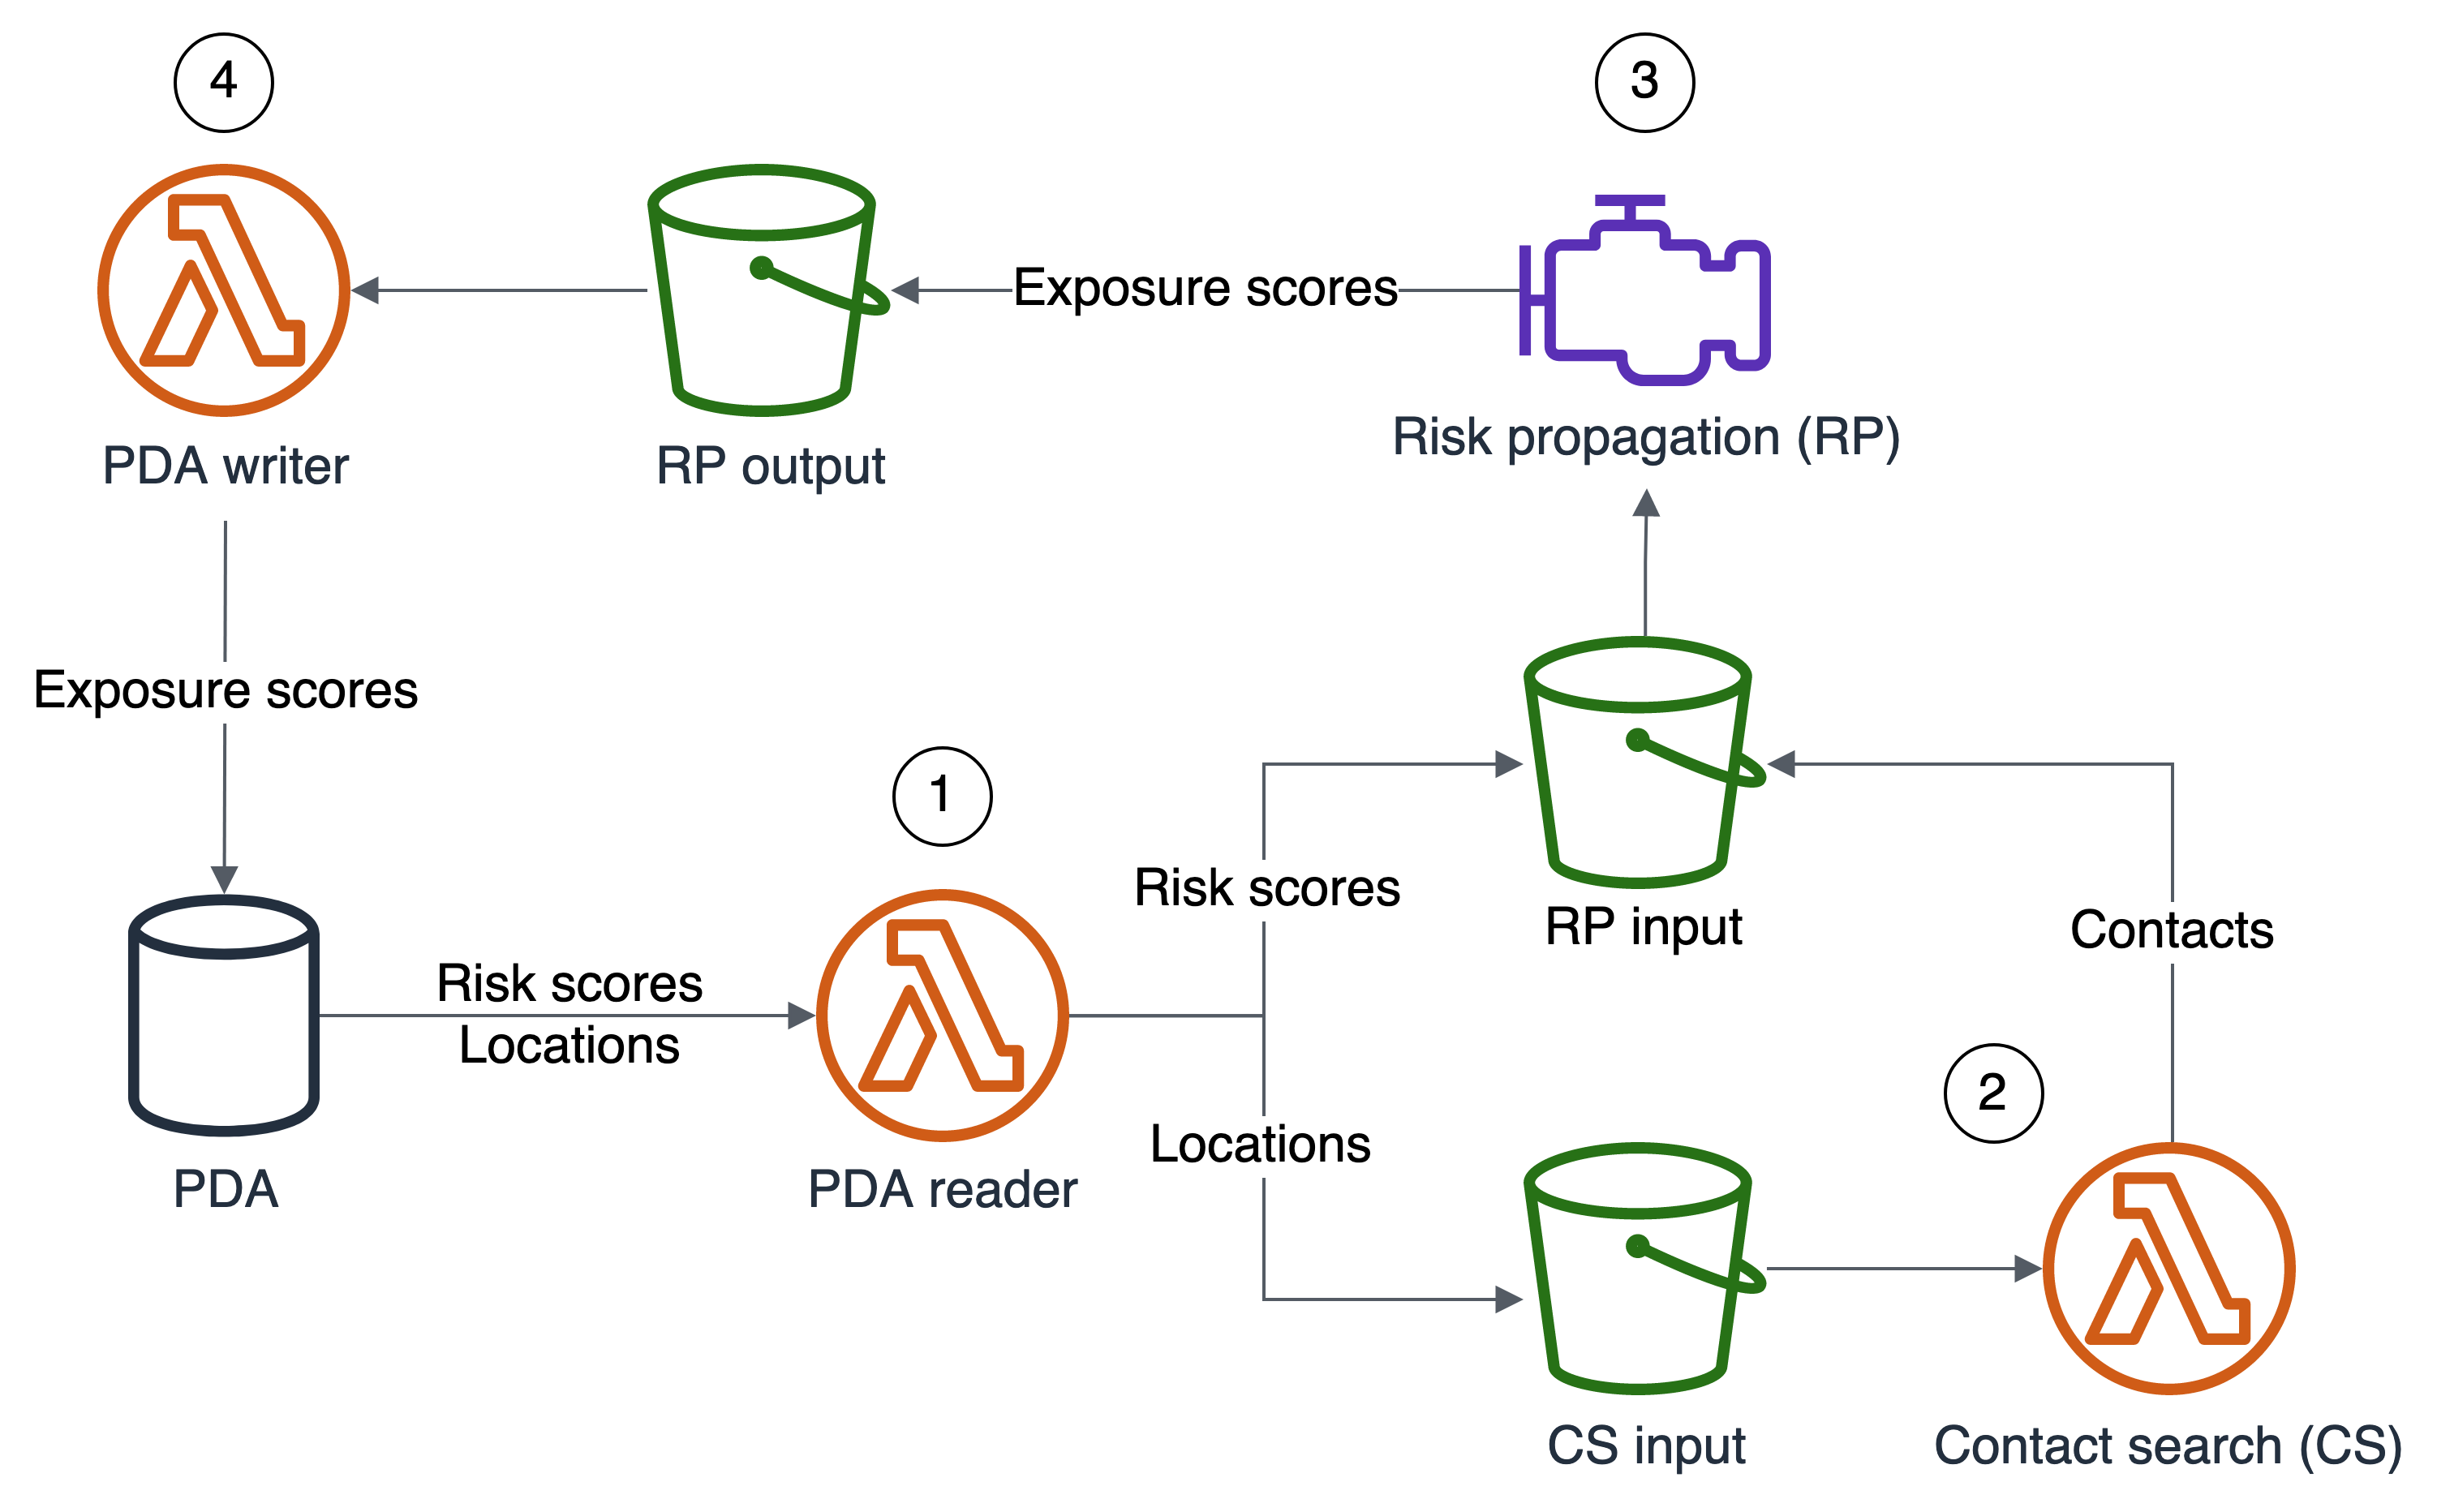
\includegraphics[width=\textwidth]{v1-architecture}
	\caption[ShareTrace batch-processing architecture]{ShareShareTrace batch-processing architecture. 
		(1) An AWS Lambda function retrieves the risk scores (symptom scores and previously computed exposure scores) and location histories from all user PDAs. Risk scores are transformed into vertex inputs for risk propagation and stored in an Amazon Simple Service (S3) bucket. Location histories are stored in a separate S3 bucket for contact extraction. (2) An AWS Lambda function executes contact search on the location histories to find all contacts, maps them to edge inputs for risk propagation, and stores them in the same S3 bucket that holds the vertex inputs. (3) Amazon Elastic MapReduce (EMR) runs risk propagation as a batch job and outputs the computed exposure scores into an S3 bucket. (4) An AWS Lambda function writes the exposure scores to the PDA of their respective user.}
	\label{fig:v1-architecture}
\end{figure}

% TODO Cite AWS Batch, S3, EMR, Lambda, Step Function
% TODO Cite fan-out pattern
\par The functionality implemented by all AWS Lambda functions was intended to follow a fan-out design in which one Lambda function would be invoked and then distribute the work amongst one or more other Lambda functions. For example, the PDA reader Lambda function would retrieve the list of all HATs and then partition that list among several other Lambda functions to retrieve user data in parallel.

\par The Giraph-based implementation is a literal interpretation of the original ShareTrace algorithm \cite{Ayday2021}. That is, it assumes a factor graph in which a factor vertex contains the contact times between two users and a variable vertex contains the maximum risk score it has received from a neighboring factor vertex. The algorithm haults when either a given number of iterations has elapsed or the total change in variable vertex values drops below a given threshold.

\par Several factors prompted the search for an alternative design to Giraph:

\begin{enumerate}
	\item \emph{Design complexity}. For a relatively straightforward data flow, the architecture in Figure \ref{fig:v1-architecture} corresponds to over 4,000 lines of source code. In retrospect, a more suitable approach than manually configured Lambda  functions would have been a managed batch-processing or workflow orchestration service, such as AWS Batch or AWS Step Function. Additionally, the low-level design of the Giraph implementation was unnecessarily complex. One-mode projection that is used in Sections \ref{sec:projected-subgraphs} and \ref{sec:vertex-actors} would have avoided the complexity of multiple vertex types. Regardless, the implementation was overengineered.
	\item \emph{Dependency management incompatability}. A major cause for redesigning the implementation was the dependency version conflicts between Giraph and the libraries used for the ShareTrace implementation. In spite of the several attempts (e.g., using different library versions, using different versions of Giraph, and forcing specific transitive dependency versions) to resolve these conflicts, a lack of personal development experience and stalled progress prompted me pursue alternatives to Giraph.
	\item \emph{Persistent data storage external to the PDA}. One of the core tenets of Dataswift is that the user fully controls the access to their data. However, as shown in Figure \ref{fig:v1-architecture}, user data is stored in S3 buckets. While it is possible to encrypt S3 objects at rest and automatically delete objects after a certain duration, data persistence to any extent is neither ideal nor desired for a privacy-preserving contact tracing solution.
\end{enumerate}

% TODO Cite Plasma object store
% TODO Cite GitHub repo after code clean up
\section{Subgraph Actors}\label{sec:subgraph-actors}

\par Attempting to mimic the design in Section \ref{sec:giraph}, I implemented risk propagation using the Python library, Ray  \cite{ray2021} that ``provides a simple, universal API for building distributed applications.'' While it claims to support actor-based programming, Ray provides relatively basic support compared to Akka, which is used in the current implementation (see Section \ref{sec:vertex-actors}). Essentially, Ray offers an extension of multiprocessing in which each actor is bound to a process. For risk propagation, I partitioned the factor graph among multiple actors such that each actor maintained a subset of variable vertices \emph{or} factor vertices. The graph topology was stored in shared memory so that it all actors could efficiently access it. The lifetime of this design was brief for the following reasons:

\begin{enumerate}
	\item \emph{Poor performance}. Interprocess communication is relatively more expensive than intraprocess communication. As a result, by partitioning the vertices such that actors only contained one type of vertex in the bipartite graph, all messages passed during risk propagation were sent to different processes. Unsurprisingly, this manifested in slow runtimes.
	\item \emph{Design complexity}. Not using a framework, like Giraph, meant that this implementation required more low-level code to implement actor functionality and message-passing. Regardless of the performance, the overall design of this implementation was poorly organized and overthought.
\end{enumerate}

\section{Monitor-Worker-Driver (MWD) Framework}\label{sec:monitor-worker}

% TODO Cite https://docs.ray.io/en/latest/ray-core/actors/patterns/tree-of-actors.html
% TODO Cite https://docs.ray.io/en/latest/ray-core/tasks/patterns/fine-grained-tasks.html
\par Based on the poor runtime performance and complexity of the approach taken in Section \ref{sec:subgraph-actors}, I speculated that centralizing the mutable aspects of risk propagation (i.e., the current value of each variable vertex) would decrease runtime and reduce the implementation complexity. With this is mind, I designed the monitor-worker-driver (MWD) framework, which draws inspiration from the tree of actors design pattern [CITE].  Figure \ref{fig:v3-architecture} describes the framework. Listing \ref{listing:v3-code} provides a partial implementation of the monitor and driver.

\begin{figure}[htbp]
	\centering
	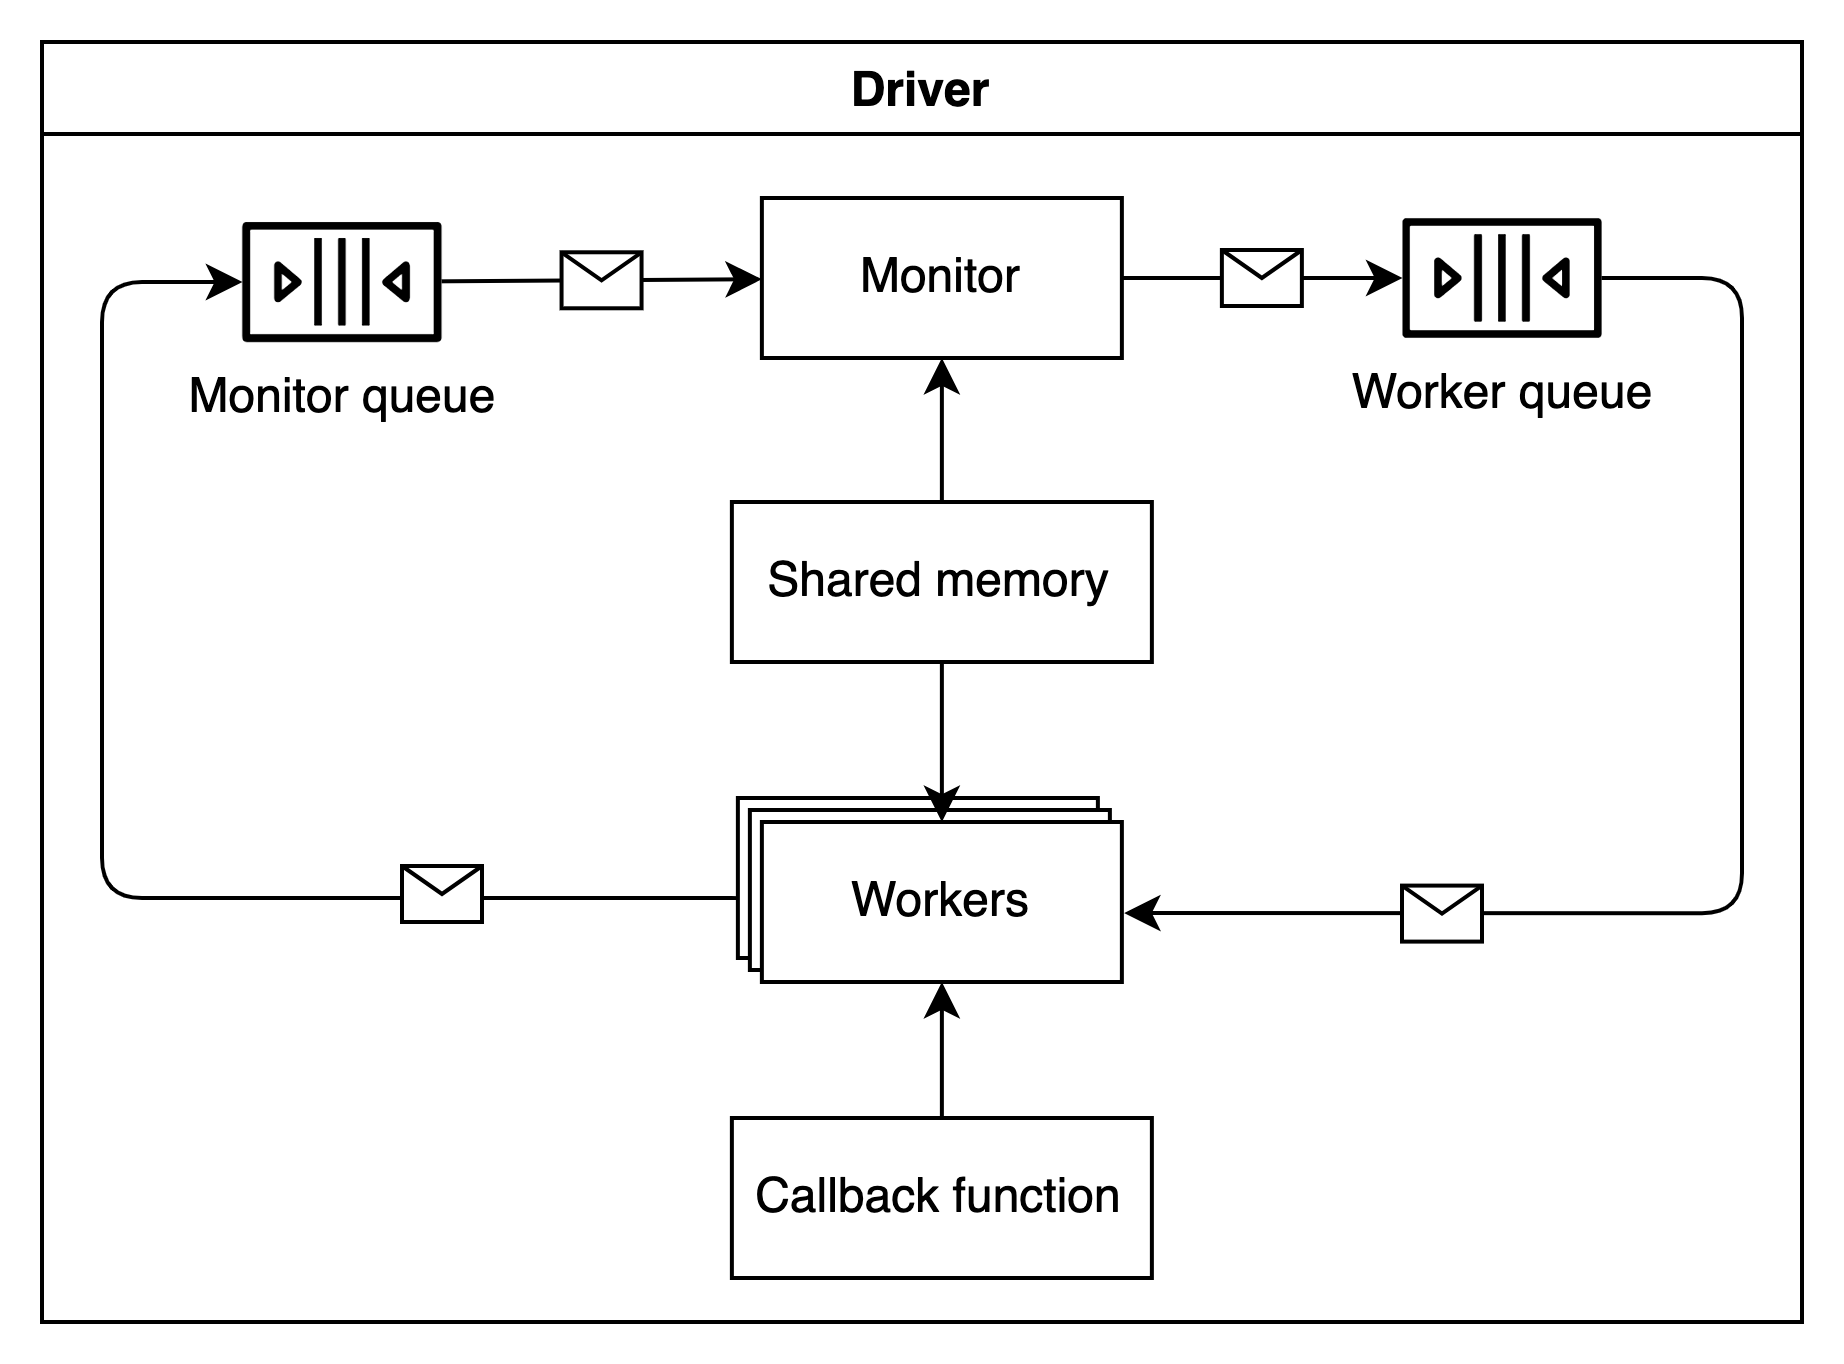
\includegraphics[width=\textwidth]{v3-architecture}
	\caption[Monitor-worker-driver framework]{Monitor-worker-driver framework.
		The \emph{monitor} is a stateful actor that is responsible for any mutable state of the program. A \emph{worker} (e.g., threads, processes, etc.) is a stateless entity that consumes monitor-produced messages from the \emph{worker queue}. Following the strategy design pattern \cite{Gamma1994}, worker behavior is defined by a \emph{callback function} which may use the attributes of a message to decide on how to process it. Any side effects of processing a message from the worker queue is encapsulated in a message and added to the \emph{monitor queue}. The monitor then consumes messages from the monitor queue, updates the state of the program, and produces messages in response for the workers to consume. The use of queues follows the mediator design pattern \cite{Gamma1994} in that the monitor and workers communicate indirectly. Any immutable state of the program can be efficiently accessed by both the monitor and the workers in \emph{shared memory}. The \emph{driver} is responsible for initiating the monitor and workers, waiting for the monitor to terminate message-passing, and returning the program output.}
	\label{fig:v3-architecture}
\end{figure}

\begin{figure}[htbp]
\centering
\begin{lstlisting}[
caption={[Monitor-worker-driver framework code]Monitor-worker framework code. The \texttt{BaseMonitor} is responsible for observing the message-passing between workers and maintaining any state of the program. The \texttt{BaseDriver} defines the rest of the message-passing program by first completing any required setup, and then returning the result from the monitor. It is composed of a worker queue instance, a monitor queue instance, a worker callback function, and the number of workers to instantiate. The type variables \texttt{Q} and \texttt{M} are used to indicate the types of the queue and message, respectively. The \texttt{BaseMonitor.call(Q, Q)} method follows the template design pattern in that it specifies the composition of multiple abstract methods and leaves their implementation to subclasses \cite{Gamma1994}.},
label=listing:v3-code]
from abc from ABC
from typing import Any, TypeVar

Q, M = TypeVar("Q"), TypeVar("M")

class BaseMonitor(ABC):
    __slots__ = ()

    def call(self, mqueue: Q, wqueue: Q) -> Any:
        while not self.should_terminate():
            # Get a message from the monitor queue.
            msg = self.get(mqueue)
            # Only process the message if necessary.
            if self.should_process(msg):
                # Optionally modify the message.
                msg = self.transform(msg)
                # Update the state of the monitor.
                self.update(msg)
                # Put the message in the worker queue.
                self.put(wqueue, msg)

class BaseDriver(ABC):
    __slots__ = "monitor", "mqueue", "wqueue", "callback", "n_workers"

    def call(self, inputs: Any) -> Any:
        # Perform any necessary setup before starting.
        self.setup(inputs)
        return self.monitor.call(self.mqueue, self.wqueue)
	\end{lstlisting}
\end{figure}

\par For risk propagation, a \texttt{RiskMonitor} monitor was implemented. It terminates when any of the following conditions are satisifed. The default behavior is to terminate once the monitor queue is empty.

\begin{itemize}
	\item The monitor has received \texttt{max\_msgs} messages.
	\item A duration of \texttt{max\_duration} has elapsed.
	\item No variable vertex has updated after \texttt{n\_msgs\_early\_stop} messages.
	\item No messages have been received \texttt{n\_retries} times after \texttt{timeout} time.
\end{itemize}

\par Only messages that are likely to induce an update to the state of the monitor are processed. The \texttt{send\_threshold} parameter allows us to vary the strictness of this likelihood. For a message sent by a variable node, the monitor only allows it if the value, scaled by \texttt{send\_threshold}, is greater than the current value of the variable vertex. This does not guarantee that it will invoke an update after the receiving factor vertex processes it, but it does prevent messages that would obviously not cause a variable vertex to update its value. Similarly, for a factor message, the monitor only allows it if the value, scaled by \texttt{send\_threshold}, is greater than the current value of the receiving variable vertex. Unlike variable messages, this guarantees against sending ineffective messages. Even if no other terminating condition is specified, the nature of \texttt{filter(M)} will gradually cause message passing to terminate. No transformation is applied to messages. The \texttt{update(M)} method contains the logic corresponding to the terminating conditions specified earlier. The monitor also updates the value of a variable vertex if the message value is greater than its current value.

\par The \texttt{RiskPropagation} driver exectutes risk propagation. Its \texttt{setup(Any)} method (1) creates the factor graph and stores it in shared memory, (2) sets the initial state of the monitor to be the maximum risk score of each variable vertex, and (3) adds all risk scores to the monitor queue. The \texttt{call(Any)} method (1) calls \texttt{setup(Any)}, (2) initializes \texttt{n\_workers} workers and the monitor, and (3) returns the state of the monitor, which is the exposure score of variable vertex.

\par Compared to the approach in Section \ref{sec:subgraph-actors}, this implementation provides a cleaner design and less communication overhead. However, what prompted me to consider (yet another) an alternative implementation was its scalability. As evidenced by Listing \ref{listing:v3-code}, the MWD framework is just a way of organizing an algorithm around the monitor while loop. Because the monitor processes messages serially, it is a bottleneck for algorithms in which the workers perform fine-grained tasks. Indeed, the Ray documentation notes that the parallelization of small tasks is an antipattern because the interprocess communication cost exceeds the benefit of multiprocessing [CITE]. Unfortunately, the functionality of a variable vertex and factor vertex is too fine-grained, so the scalability of the MWD framework is no better than a serial implementation.

% TODO
\section{Subgraph Actors with Projection}\label{sec:projected-subgraphs}

Improvements:
1. Best functioning implementation thus far 

Drawbacks:
1. Heavily dependent on the graph partitioning

% TODO
\section{Thinking Like a Vertex with Actors}\label{sec:vertex-actors}

Improvements:
1. Distributed; a drawback of all but the first approach
2. Decentralized; a drawback of all previous approaches
3. Robust; allows for delays in the changes of the contact graph with caching
4. Scalable and performant

Drawbacks:
1. Concurrent execution is difficult to reason about
%%% This defines the bibliography file (main.bib) and the bibliography style.
%% If you want to create a bibliography file by hand, change the contents of
%% this file to a `thebibliography' environment.  For more information 
%% see section 4.3 of the LaTeX manual.
\begin{singlespace}
\bibliography{main}
\bibliographystyle{plain}
\end{singlespace}

\end{document}

